\section{Parallel Patterns}

\begin{itemize}
    \item Nesting Pattern
\end{itemize}

\subsection{Serial Control Patterns}


sequence,selection,iteration,recursion

\subsection{Parallel Control Pattern}

fork-join,map,stencil,reduction,scan, recurrence

\subsection{Serial DATA management Patterns}

random read and write, stack allocation, heap allocation, objects.

\subsection{Parallel Data Management Patterns}

pack, pipeline, geometric decomposition, gather, scatter.

\section{Depencencias}

\textbf{Sequential Consistency in Parallel Exectuion}, Statments exectuion does not interfere with each other, Computations result equal to either A B or B A \par

\textbf{True Dependency} - Read After Write $\delta$ \par
\textbf{Anti-Dependence} - Write After Read $\delta^{-1}$\par
\textbf{Output Dependence} - Write After Write $\delta^{0}$\par

Some dependences can be removed by modifying the program. - Rearranging statements and or Eliminating statements.\par

Loop Carried dependence is a dependence between two statements instances in two different iterations of a loop. Otherwise, it is loop-independent.

\section{Map Reduce}

a program model and a an associated implementation for processing large databasets.\par
Batch processing: - All input in know when the computation starts, the complete computation is executed, No interaction with the user.\par

\begin{enumerate}
    \item Record Reader
    \item Map
    \item Combiner (Optional)
    \item Partioner
    \item Shuffle and Sort
    \item Reduce
\end{enumerate}

\section{Synchronization}

Sequencial Algorithm -> formal description of a behavior of a sequential state machine. When written in a specific programming language. an algorithm is called a program. A process is an instance of an algorithm.\par

\textbf{Competition} : To access to the disk resource\par
\textbf{Cooperation} : Barrier, producer-consumer

\subsection{Solving Mutual Exclusion}
\textbf{Atomic Register}\par 

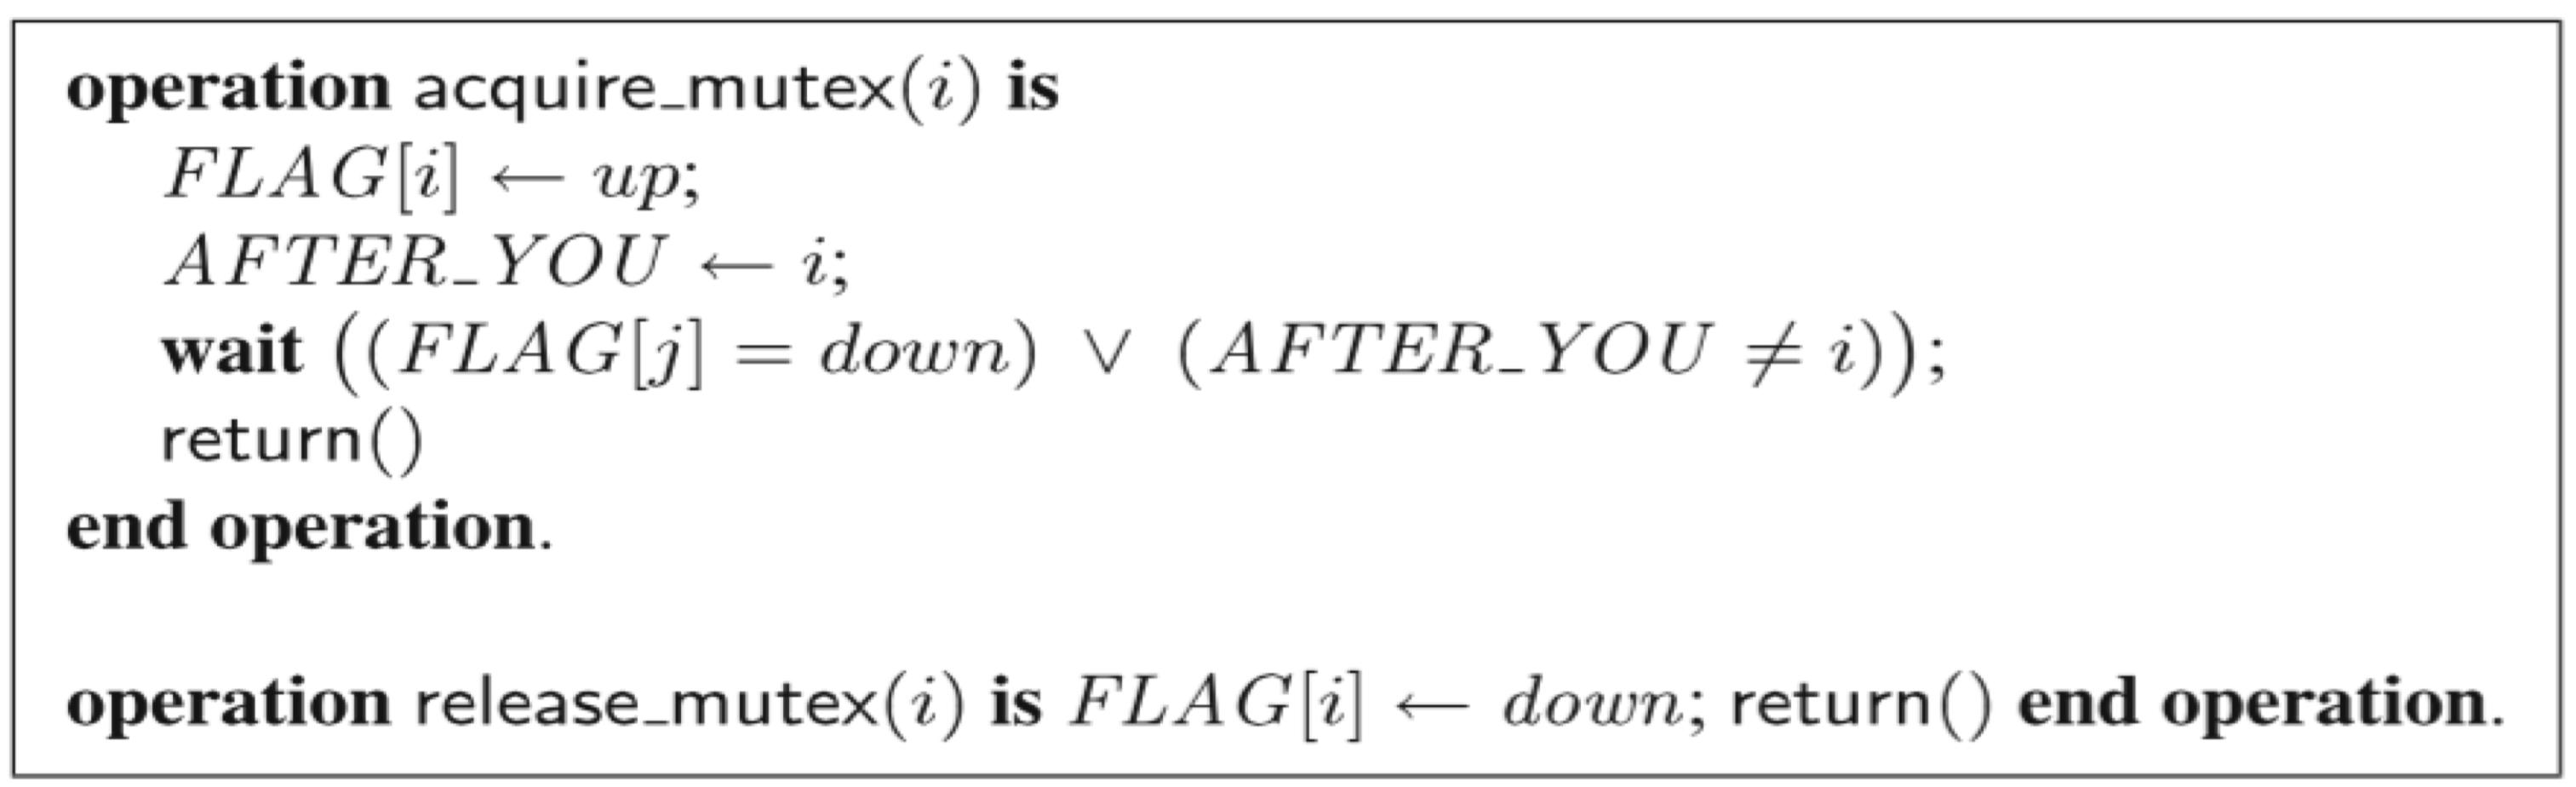
\includegraphics[width=\linewidth]{img/ema.png}

\textbf{Special hardware primitives}\par

test\&set / reset \par
swap \par
compare\&swap\par
fetch\&add

\section{Locking Strategies}

\subsection{Coarse-Grained Synchronization}
Use a single lock. Methods executed in mutual exclusion.\par
Eliminates all the concurrency within the object.

\subsection{Fine-Grained Synchronization}
(Hand-over hand locking, linked list)\par
Split object intomultiple independenty-synchronized components.\par
Methods conflict when they access the same component at the same time.

\subsection{Optimistic Synchronization}
Check if the operation can be done if so, lock and check again.\par
Traverse the list without locking until location is found. Lock nodes and transverse again to confirm that the locked nodes are still in the list.

\subsection{Lazy Synchronization}
Pospone Hard Work (Logical removal, Physical removal containers are wait-free)

\subsection{Lock-Free Synchronization}
Compare and Set reference and deleted bit at the some time. (In java use,)